Wir betrachten hier einige Testfunktionen, die als Zielfunktion
verschiedener restringierter Optimierungsaufgaben benutzt werden k�nnen.

\begin{testfunction}
Quadratische Funktion in $\R^n$
\[
  f(x) := \| x - d \|^2 = \sum_{k=1}^{n} (x_k - d_k)^2
\]
\end{testfunction}
Die erste Testfunktion ist eine einfache mehrdimensionale Parabel
mit Minimalstelle im Punkt~$d$ und Optimalwert~0.

\begin{testfunction}
Exponentielle Funktion
\[
  f(x) := e^{\|x\|^2} = e^{\sum_{k=1}^{n} x_k^2}
\]
\end{testfunction}
\begin{figure}[ht]
  \centering
  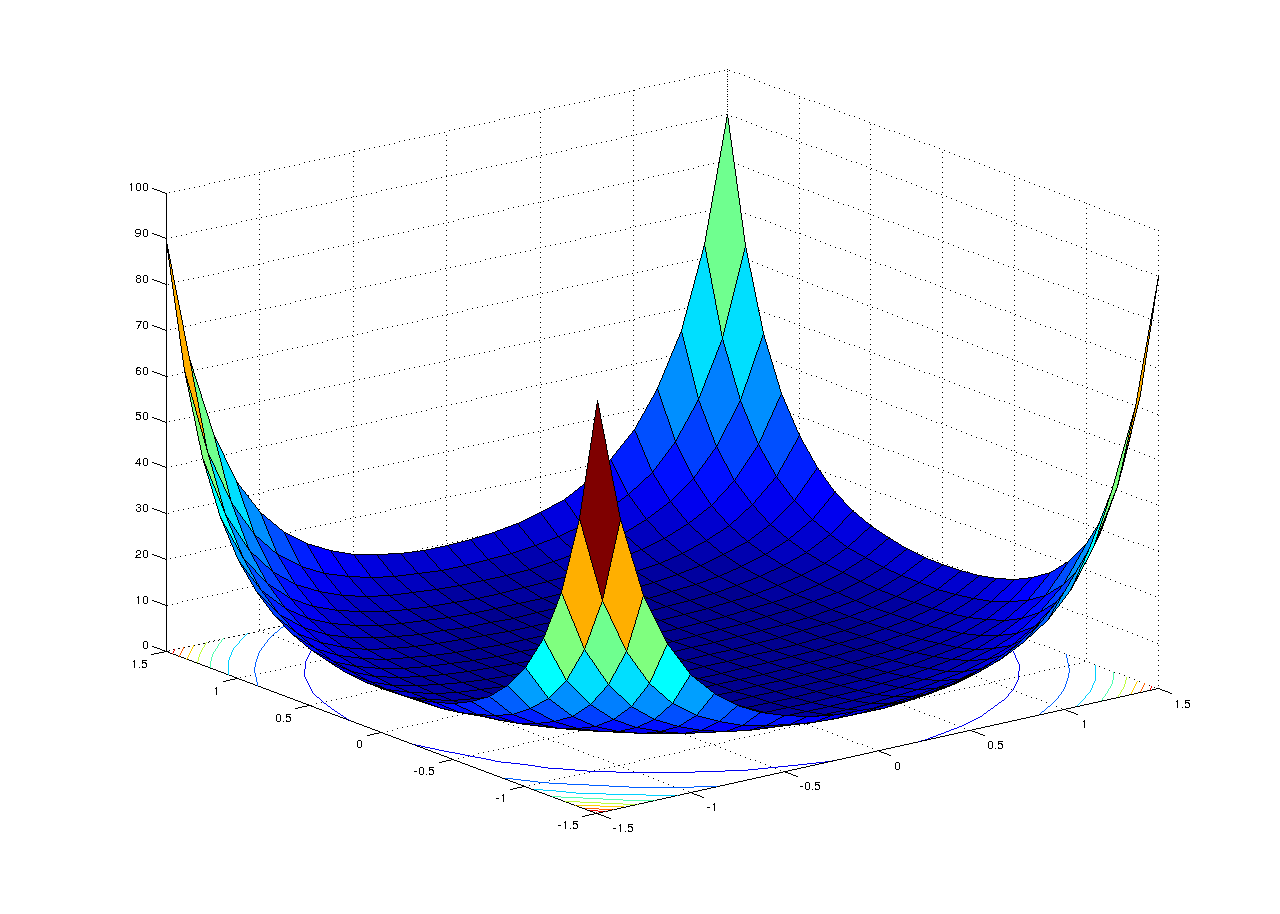
\includegraphics[width=0.75\textwidth]{exp-func}
  \caption{Exponentielle Funktion}
  \label{fig:exp_func}
\end{figure}
Die zweite Testfunktion ist eine exponentielle Funktion
mit Minimalstelle im Ursprung und Optimalwert~1.
Diese Funktion ist herausfordend, weil ihre Funktionswerte sehr schnell
gro� werden k�nnen.

\begin{testfunction}
Rosenbrock-Funktion (vgl. Beispiel 1.4.1 in \cite[S.~14]{alt})
\[
  f(x) := 100(x_2-x_1^2)^2+(1-x_1)^2
\]
\end{testfunction}
\begin{figure}[ht]
  \centering
  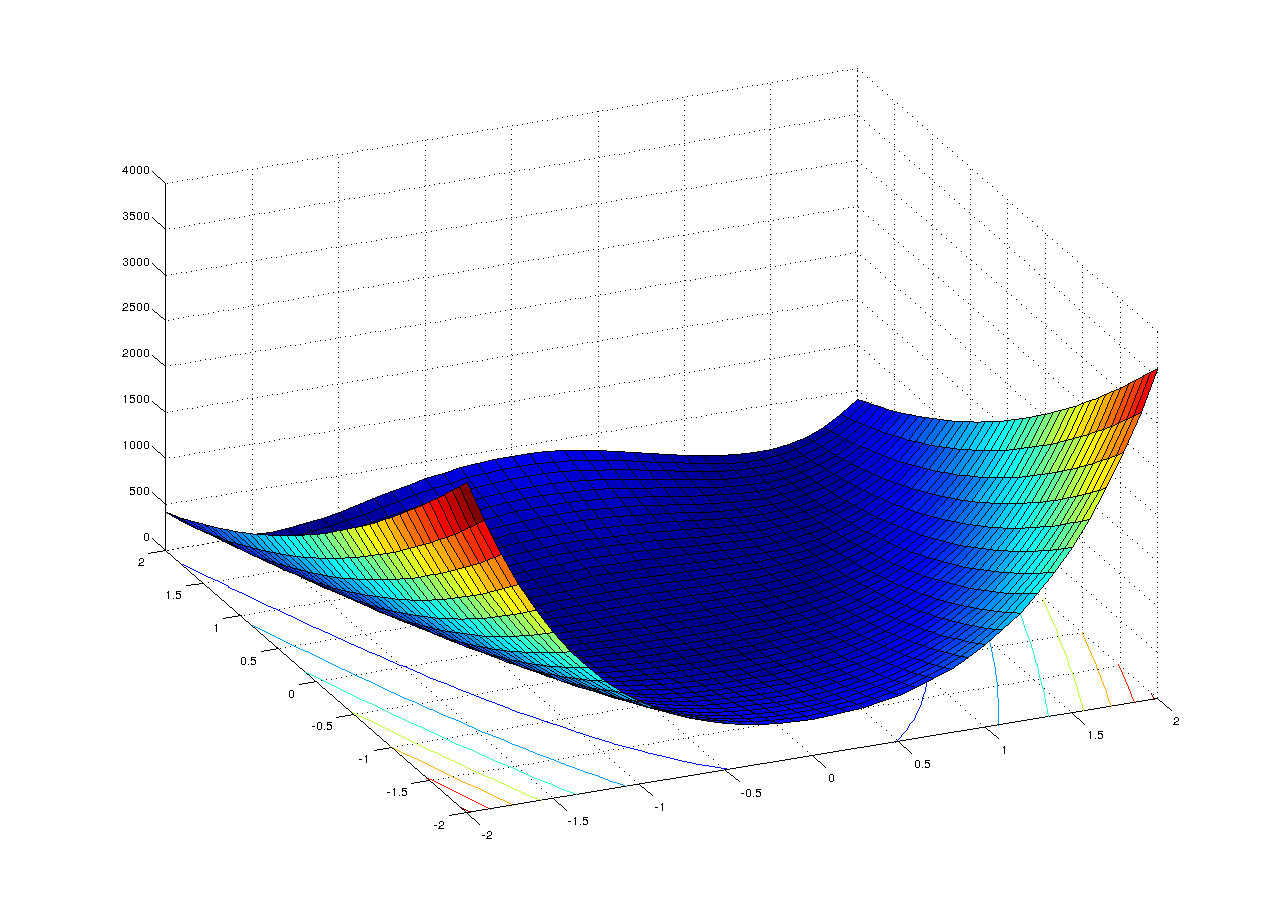
\includegraphics[width=0.75\textwidth]{rosenbrock}
  \caption{Rosenbrock-Funktion}
  \label{fig:rosenbrock}
\end{figure}
Die Rosenbrock-Funktion hat ein einziges Minimum
an der Stelle $\xopt = (1,1)^T$ mit $f(\xopt) = 0$.
Diese Funktion kann f�r manche Verfahren Schwierigkeiten anbieten,
da ihr Minimum in einem schmalen "`bananenf�rmig"' gekr�mmten Tal liegt.
Als Anfangspunkt wird normalerweise den Punkt $x^0 = (-1,1)^T$ genommen.

\begin{testfunction}
Himmelblau-Funktion (vgl. Beispiel 1.4.2 in \cite[S.~14f]{alt})
\[
  f(x) := (x_1^2+x_2-11)^2 + (x_1+x_2^2-7)^2
\]
\end{testfunction}
\begin{figure}[ht]
  \centering
  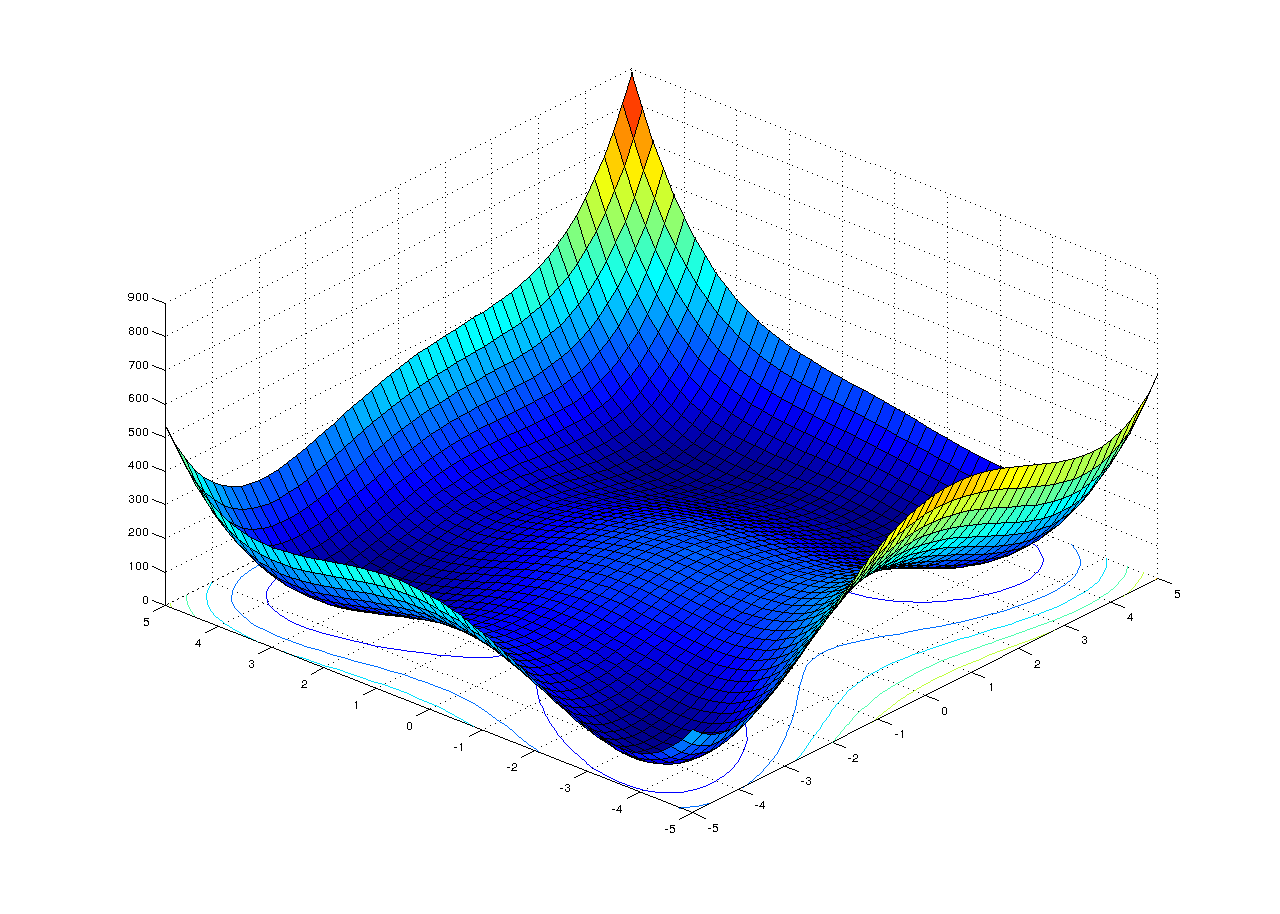
\includegraphics[width=0.75\textwidth]{himmelblau}
  \caption{Himmelblau-Funktion}
  \label{fig:himmelblau}
\end{figure}
Die Himmelblau-Funktion ist ein Polynom 4.~Grades
mit vier globale Minimalstellen.
Ein Minimum ist z.\,B. an der Stelle $\xopt = (3,2)^T$.
Der Optimalwert ist 0.

\begin{testfunction}
Bazaraa-Shetty-Funktion (vgl. Beispiel 1.4.3 in \cite[S.~15f]{alt})
\[
  f(x) := (x_1-2)^4+(x_1-2x_2)^2
\]
\end{testfunction}
\begin{figure}[ht]
  \centering
  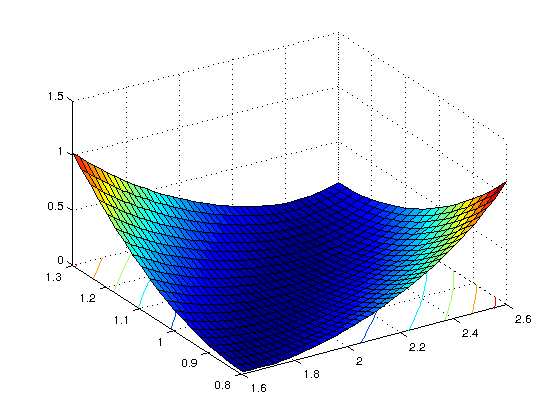
\includegraphics[width=0.75\textwidth]{bazaraa-shetty}
  \caption{Bazaraa-Shetty-Funktion}
  \label{fig:bazaraa_shetty}
\end{figure}
Die Bazaraa-Shetty-Funktion ist ein Polynom 4.~Grades
mit einem globalen Minimum in $\xopt = (2,1)^T$
und Optimalwert 0.

\begin{testfunction}
(vgl. Beispiel 1.4.4 in \cite[S.~16]{alt})
\[
  f(x_1,\ldots,x_5) := 2x_1^2 + 2x_2^2 + x_3^2
    + x_4^2 + \tfrac{1}{2}x_5^2 - 4x_1 - 4x_2 - 2x_3
      - 2x_4 - x_5 + 6\tfrac{1}{2}
\]
\end{testfunction}
Diese quadratische Funktion hat ein globales Minimum
an der Stelle $\xopt = (1,1,1,1,1)^T$ mit $f(\xopt) = 0$.

\begin{testfunction}
Dixon-Funktion (vgl. Beispiel 1.4.5 in \cite[S.~16]{alt})
\[
(1-x_1)^2 + \sum_{k=1}^{9} (x_k^2-x_{k+1})^2 + (1-x_{10})^2
\]
\end{testfunction}
Die Dixon-Funktion ist ein Polynom 4.~Grades mit 10 Variablen.
Das globale Minimum ist an der Stelle $\xopt = (1,\ldots,1)^T$
und hat den Optimalwert 0.

\begin{testfunction}
Beale-Funktion (vgl. Aufgabe 2.2 in \cite[S.~39]{alt})
\[
  f(x) := (1.5 - x_1(1-x_2))^2
    + (2.25 - x_1(1-x_2^2))^2 + (2.625 - x_1(1-x_2^3))^2
\]
\end{testfunction}
Das globale Minimum ist an der Stelle $\xopt = (3,0.5)^T$.

\begin{testfunction}
Colville-Funktion
\begin{multline}
  f(x) := 100(x_2-x_1^2)^2 + (1-x_1)^2 + 90(x_4-x_3^2)^2 + (1-x_3)^2 \\
    + 10.1((x_2-1)^2 + (x_4-1)^2) + 19.8(x_2-1)(x_4-1) \notag
\end{multline}
\end{testfunction}
Die Colville-Funktion ist ein Polynom 4.~Grades mit vier Variablen.
Das globale Minimum ist in $\xopt = (1,1,1,1)^T$ und Optimalwert 0.
